\documentclass[11pt,oneside]{article}
\usepackage[T1]{fontenc}
\usepackage[utf8]{inputenc}
% \usepackage{lmodern}
%\usepackage[adobe-utopia,uppercase=upright,greeklowercase=upright]{mathdesign}
\usepackage[adobe-utopia]{mathdesign}
%\usepackage{minionpro}
% \usepackage{pifont}
% \usepackage{amssymb}
\usepackage{amsmath}
\usepackage[francais]{babel}
% \usepackage[francais]{varioref}
\usepackage[dvips]{graphicx}

\usepackage{framed}
\usepackage[normalem]{ulem}
\usepackage{fancyhdr}
\usepackage{titlesec}
\usepackage{vmargin}
\usepackage{longtable}

\usepackage{ifthen}


%\usepackage{epsfig}
\usepackage{subfig}

\usepackage{multirow}
\usepackage{multicol} % Portions de texte en colonnes
\usepackage{flafter}%floatants après la référence



\usepackage{color}
\usepackage{colortbl}


\definecolor{gris25}{gray}{0.75}
\definecolor{bleu}{RGB}{18,33,98}
\definecolor{bleuf}{RGB}{42,94,171}
\definecolor{bleuc}{RGB}{231,239,247}
\definecolor{rougef}{RGB}{185,18,27}
\definecolor{rougec}{RGB}{255,230,231}
\definecolor{vertf}{RGB}{103,126,82}
\definecolor{vertc}{RGB}{220,255,191}

\newenvironment{rem}[1][\hsize]%
{%
    \def\FrameCommand
    {%
\rotatebox{90}{\textit{\textsf{Remarque}}} 
        {\color{bleuf}\vrule width 3pt}%
        \hspace{0pt}%must no space.
        \fboxsep=\FrameSep\colorbox{bleuc}%
    }%
    \MakeFramed{\hsize#1\advance\hsize-\width\FrameRestore}%
}%
{\endMakeFramed}%


\newenvironment{savoir}[1][\hsize]%
{%
    \def\FrameCommand
    {%
\rotatebox{90}{\textit{\textsf{Savoir}}} 
        {\color{bleuf}\vrule width 3pt}%
        \hspace{0pt}%must no space.
        \fboxsep=\FrameSep\colorbox{bleuc}%
    }%
    \MakeFramed{\hsize#1\advance\hsize-\width\FrameRestore}%
}%
{\endMakeFramed}%

\newenvironment{prob}[1][\hsize]%
{%
    \def\FrameCommand%
    {%
\rotatebox{90}{\textit{\textsf{ Problématique}}} 
        {\color{rougef}\vrule width 3pt}%
        \hspace{0pt}%must no space.
        \fboxsep=\FrameSep\colorbox{rougec}%
    }%
    \MakeFramed{\hsize#1\advance\hsize-\width\FrameRestore}%
}%
{\endMakeFramed}%

\newenvironment{obj}[1][\hsize]%
{%
    \def\FrameCommand%
    {%
\rotatebox{90}{\textit{\textsf{ $\;$}}} 
        {\color{rougef}\vrule width 3pt}%
        \hspace{0pt}%must no space.
        \fboxsep=\FrameSep\colorbox{rougec}%
    }%
    \MakeFramed{\hsize#1\advance\hsize-\width\FrameRestore}%
}%
{\endMakeFramed}%

\newenvironment{defi}[1][\hsize]%
{%
    \def\FrameCommand%
    {%
\rotatebox{90}{\textit{\textsf{Définition\\}}} 
        {\color{bleuf}\vrule width 3pt}%
        \hspace{0pt}%must no space.
        \fboxsep=\FrameSep\colorbox{bleuc}%
    }%
    \MakeFramed{\hsize#1\advance\hsize-\width\FrameRestore}%
}%
{\endMakeFramed}%


\newenvironment{hypo}[1][\hsize]%
{%
    \def\FrameCommand%
    {%
\rotatebox{90}{\textit{\textsf{Hypothèse\\}}} 
        {\color{bleuf}\vrule width 3pt}%
        \hspace{0pt}%must no space.
        \fboxsep=\FrameSep\colorbox{bleuc}%
    }%
    \MakeFramed{\hsize#1\advance\hsize-\width\FrameRestore}%
}%
{\endMakeFramed}%


\newenvironment{prop}[1][\hsize]%
{%
    \def\FrameCommand%
    {%
\rotatebox{90}{\textit{\textsf{Propriété\\}}} 
        {\color{bleuf}\vrule width 3pt}%
        \hspace{0pt}%must no space.
        \fboxsep=\FrameSep\colorbox{bleuc}%
    }%
    \MakeFramed{\hsize#1\advance\hsize-\width\FrameRestore}%
}%
{\endMakeFramed}%

\newenvironment{props}[1][\hsize]%
{%
    \def\FrameCommand%
    {%
\rotatebox{90}{\textit{\textsf{Propriétés\\}}} 
        {\color{bleuf}\vrule width 3pt}%
        \hspace{0pt}%must no space.
        \fboxsep=\FrameSep\colorbox{bleuc}%
    }%
    \MakeFramed{\hsize#1\advance\hsize-\width\FrameRestore}%
}%
{\endMakeFramed}%

\newenvironment{exemple}[1][\hsize]%
{%
    \def\FrameCommand%
    {%
\rotatebox{90}{\textit{\textsf{Exemple\\}}} 
        {\color{vertf}\vrule width 3pt}%
        \hspace{0pt}%must no space.
        \fboxsep=\FrameSep\colorbox{vertc}%
    }%
    \MakeFramed{\hsize#1\advance\hsize-\width\FrameRestore}%
}%
{\endMakeFramed}%

\newenvironment{resultat}[1][\hsize]%
{%
    \def\FrameCommand%
    {%
\rotatebox{90}{\textit{\textsf{Résultat\\}}} 
        {\color{rougef}\vrule width 3pt}%
        \hspace{0pt}%must no space.
        \fboxsep=\FrameSep\colorbox{rougec}%
    }%
    \MakeFramed{\hsize#1\advance\hsize-\width\FrameRestore}%
}%
{\endMakeFramed}%

\newenvironment{methode}[1][\hsize]%
{%
    \def\FrameCommand%
    {%
\rotatebox{90}{\textit{\textsf{Méthode\\}}} 
        {\color{rougef}\vrule width 3pt}%
        \hspace{0pt}%must no space.
        \fboxsep=\FrameSep\colorbox{rougec}%
    }%
    \MakeFramed{\hsize#1\advance\hsize-\width\FrameRestore}%
}%
{\endMakeFramed}%

\newenvironment{theo}[1][\hsize]%
{%
    \def\FrameCommand%
    {%
\rotatebox{90}{\textit{\textsf{Théorème\\}}} 
        {\color{rougef}\vrule width 3pt}%
        \hspace{0pt}%must no space.
        \fboxsep=\FrameSep\colorbox{rougec}%
    }%
    \MakeFramed{\hsize#1\advance\hsize-\width\FrameRestore}%
}%
{\endMakeFramed}%

\newenvironment{warn}[1][\hsize]%
{%
    \def\FrameCommand%
    {%
\rotatebox{90}{\textit{\textsf{Attention\\}}} 
        {\color{rougef}\vrule width 3pt}%
        \hspace{0pt}%must no space.
        \fboxsep=\FrameSep\colorbox{rougec}%
    }%
    \MakeFramed{\hsize#1\advance\hsize-\width\FrameRestore}%
}%
{\endMakeFramed}%

% \usepackage{pstricks}
%\usepackage{minitoc}
% \setcounter{minitocdepth}{4}

\setcounter{tocdepth}{2}

% \mtcselectlanguage{french} 

%\usepackage{draftcopy}% "Brouillon"
% \usepackage{floatflt}
\usepackage{psfrag}
%\usepackage{listings} % Permet d'insérer du code de programmation
\renewcommand{\baselinestretch}{1.2}

% Changer la numérotation des figures :
% ------------------------------------
% \makeatletter
% \renewcommand{\thefigure}{\ifnum \c@section>\z@ \thesection.\fi
%  \@arabic\c@figure}
% \@addtoreset{figure}{section}
% \makeatother
 


%%%%%%%%%%%%
% Définition des vecteurs %
%%%%%%%%%%%%
 \newcommand{\vect}[1]{\overrightarrow{#1}}

%%%%%%%%%%%%
% Définition des torseusr %
%%%%%%%%%%%%

 \newcommand{\torseur}[1]{%
\left\{{#1}\right\}
}

\newcommand{\torseurcin}[3]{%
\left\{\mathcal{#1} \left(#2/#3 \right) \right\}
}

\newcommand{\torseurstat}[3]{%
\left\{\mathcal{#1} \left(#2\rightarrow #3 \right) \right\}
}

 \newcommand{\torseurc}[8]{%
%\left\{#1 \right\}=
\left\{
{#1}
\right\}
 = 
\left\{%
\begin{array}{cc}%
{#2} & {#5}\\%
{#3} & {#6}\\%
{#4} & {#7}\\%
\end{array}%
\right\}_{#8}%
}

 \newcommand{\torseurcol}[7]{
\left\{%
\begin{array}{cc}%
{#1} & {#4}\\%
{#2} & {#5}\\%
{#3} & {#6}\\%
\end{array}%
\right\}_{#7}%
}

 \newcommand{\torseurl}[3]{%
%\left\{\mathcal{#1}\right\}_{#2}=%
\left\{%
\begin{array}{l}%
{#1} \\%
{#2} %
\end{array}%
\right\}_{#3}%
}

 \newcommand{\vectv}[3]{%
\vect{V\left( {#1} \in {#2}/{#3}\right)}
}


\newcommand{\vectf}[2]{%
\vect{R\left( {#1} \rightarrow {#2}\right)}
}

\newcommand{\vectm}[3]{%
\vect{\mathcal{M}\left( {#1}, {#2} \rightarrow {#3}\right)}
}


 \newcommand{\vectg}[3]{%
\vect{\Gamma \left( {#1} \in {#2}/{#3}\right)}
}

 \newcommand{\vecto}[2]{%
\vect{\Omega\left( {#1}/{#2}\right)}
}
% }$$\left\{\mathcal{#1} \right\}_{#2} =%
% \left\{%
% \begin{array}{c}%
%  #3 \\%
%  #4 %
% \end{array}%
% \right\}_{#5}}

%  ------------------------------------------
% | Modification du formatage des sections : | 
%  ------------------------------------------

% Grands titres :
% ---------------

\newcommand{\titre}[1]{%
\begin{center}
      \bigskip
      \rule{\textwidth}{1pt}
      \par\vspace{0.1cm}
      
      \textbf{\large #1}
      \par\rule{\textwidth}{1pt}
    \end{center}
    \bigskip
  }

% Supprime le numéro du chapitre dans la numérotation des sections:
% -----------------------------------------------------------------
\makeatletter
\renewcommand{\thesection}{\@arabic\c@section}
\makeatother


% \titleformat{\chapter}[display]
% {\normalfont\Large\filcenter}
% {}
% {1pc}
% {\titlerule[1pt]
%   \vspace{1pc}%
%   \Huge}[\vspace{1ex}%
% \titlerule]


%%%% Chapitres Comme PY Pechard %%%%%%%%%
% numéro du chapitre
\DeclareFixedFont{\chapnumfont}{OT1}{phv}{b}{n}{80pt}
% pour le mot « Chapitre »
\DeclareFixedFont{\chapchapfont}{OT1}{phv}{m}{it}{40pt}
% pour le titre
\DeclareFixedFont{\chaptitfont}{T1}{phv}{b}{n}{25pt}

\definecolor{gris}{gray}{0.75}
\titleformat{\chapter}[display]%
	{\sffamily}%
	{\filleft\chapchapfont\color{gris}\chaptertitlename\
	\\
	\vspace{12pt}
	\chapnumfont\thechapter}%
	{16pt}%
	{\filleft\chaptitfont}%
	[\vspace{6pt}\titlerule\titlerule\titlerule]

%%%%  Fin Chapitres Comme PY Pechard %%%%%%%%%


% Section, subsection, subsubsection sans serifs :
% % ----------------------------------------------

% \makeatletter
% \renewcommand{\section}{\@startsection{section}{0}{0mm}%
% {\baselineskip}{.3\baselineskip}%
% {\normalfont\sffamily\Large\textbf}}%
% \makeatother

\makeatletter
\renewcommand{\@seccntformat}[1]{{\textcolor{bleu}{\csname
the#1\endcsname}\hspace{0.5em}}}
\makeatother

\makeatletter
\renewcommand{\section}{\@startsection{section}{1}{\z@}%
                       {-4ex \@plus -1ex \@minus -.4ex}%
                       {1ex \@plus.2ex }%
                       {\normalfont\Large\sffamily\bfseries}}%
\makeatother
 
\makeatletter
\renewcommand{\subsection}{\@startsection {subsection}{2}{\z@}
                          {-3ex \@plus -0.1ex \@minus -.4ex}%
                          {0.5ex \@plus.2ex }%
                          {\normalfont\large\sffamily\bfseries}}
\makeatother
 
\makeatletter
\renewcommand{\subsubsection}{\@startsection {subsubsection}{3}{\z@}
                          {-2ex \@plus -0.1ex \@minus -.2ex}%
                          {0.2ex \@plus.2ex }%
                          {\normalfont\large\sffamily\bfseries}}
\makeatother
 
\makeatletter             
\renewcommand{\paragraph}{\@startsection{paragraph}{4}{\z@}%
                                    {-2ex \@plus-.2ex \@minus .2ex}%
                                    {0.1ex}%               
{\normalfont\sffamily\bfseries}}
\makeatother
 
\makeatletter
\renewcommand{\subparagraph}{\@startsection{subparagraph}{5}{\z@}%
                                       {-2ex \@plus-.1ex \@minus .2ex}%
                                       {0.1ex}%
				    {\normalfont\normalsize\sffamily\bfseries}}
\makeatletter
% \makeatletter
% \renewcommand{\subsection}{\@startsection{subsection}{1}{2mm}%
% {\baselineskip}{.3\baselineskip}%
% {\normalfont\sffamily\large\textbf}}%
% \makeatother
% 
% \makeatletter
% \renewcommand{\subsubsection}{\@startsection{subsubsection}{2}{4mm}%
% {\baselineskip}{.15\baselineskip}%
% {\normalfont\sffamily\large\textbf}}%
% \makeatother
% 
% \makeatletter
% \renewcommand{\paragraph}{\@startsection{paragraph}{3}{6mm}%
% {\baselineskip}{.15\baselineskip}%
% {\normalfont\sffamily\large\textbf}}%
% \makeatother
 
\setcounter{secnumdepth}{4}


%  --------
% | Marges |
%  --------


% \setmarginsrb{2.5cm}{1.5cm}{2.5cm}{2cm}{1cm}{1cm}{1cm}{1cm}
\setmarginsrb{1.5cm}{1cm}{1cm}{1.5cm}{1cm}{1cm}{1cm}{1cm}

% Changer les marges localement :
% -----------------------------
\newenvironment{changemargin}[2]{\begin{list}{}{%
\setlength{\topsep}{0pt}%
\setlength{\leftmargin}{0pt}%
\setlength{\rightmargin}{0pt}%
\setlength{\listparindent}{\parindent}%
\setlength{\itemindent}{\parindent}%
\setlength{\parsep}{0pt plus 1pt}%
\addtolength{\leftmargin}{#1}%
\addtolength{\rightmargin}{#2}%
}\item }{\end{list}}



\usepackage{pst-solides3d}
\usepackage{titletoc}
\titlecontents{chapter}[+3pc]
  {\addvspace{10pt}\sffamily\bfseries}
{\contentslabel[{\pscirclebox[fillstyle=solid,fillcolor=gray!25,
linecolor=gray!25,framesep=4pt]{\textcolor{white}{\thecontentslabel}}}]{2.5pc}}
  {}
  {\dotfill \normalfont\thecontentspage\ }

\titlecontents{section}[3pc]
  {\addvspace{2pt}\sffamily}
  {\contentslabel[\thecontentslabel]{1.8pc}}
  {}
  {\dotfill \normalfont\thecontentspage\ }

\titlecontents{subsection}[5pc]
  {\addvspace{2pt}\sffamily}
  {\contentslabel[\thecontentslabel]{1.8pc}}
  {}
  {\dotfill \normalfont\thecontentspage\ }

\titlecontents{subsubsection}[8pc]
  {\addvspace{2pt}\sffamily}
  {\contentslabel[\thecontentslabel]{3pc}}
  {}
  {\dotfill \normalfont\thecontentspage\ }
%{\;\titlerule\;\normalfont\thecontentspage\ }

\titlecontents{paragraph}[9pc]
  {\addvspace{2pt}\sffamily}
  {\contentslabel[\thecontentslabel]{3.5pc}}
  {}
  {\dotfill \normalfont\thecontentspage\ }



\usepackage[raccourcis]{FAST}
\usepackage[%
    pdftitle={Produits Procédés Matériaux -- },
    pdfauthor={Xavier Pessoles},
    colorlinks=true,
    linkcolor=blue,
    citecolor=magenta]{hyperref}
\usepackage{schemabloc}



% \makeatletter \let\ps@plain\ps@empty \makeatother
%% DEBUT DU DOCUMENT
%% =================
\sloppy
\hyphenpenalty 10000

\newcommand{\Pointilles}[1][3]{%
\multido{}{#1}{\makebox[\linewidth]{\dotfill}\\[\parskip]
}}


\colorlet{shadecolor}{orange!15}

\newtheorem{theorem}{Theorem}


\begin{document}


\newboolean{prof}
\setboolean{prof}{true}
%------------- En tetes et Pieds de Pages ------------
\pagestyle{fancy}
\renewcommand{\headrulewidth}{0pt}

\fancyhead{}
\fancyhead[L]{%
\noindent\noindent\begin{minipage}[c]{2.6cm}
%Lycée Rouvière PTSI

\includegraphics[width=2cm]{png/logo_ptsi.png}%
\end{minipage}
}

\fancyhead[C]{\rule{12cm}{.5pt}}

\fancyhead[R]{%
\noindent\begin{minipage}[c]{3cm}
\begin{flushright}
\footnotesize{\textit{\textsf{Sciences Industrielles\\ pour l'Ingénieur}}}%
\end{flushright}
\end{minipage}
}

\renewcommand{\footrulewidth}{0.2pt}

\fancyfoot[C]{\footnotesize{\bfseries \thepage}}
\fancyfoot[L]{\footnotesize{2012 -- 2013} \\ X. \textsc{Pessoles}}
\ifthenelse{\boolean{prof}}{%
\fancyfoot[R]{\footnotesize{Cours -- CI 6 : PPM -- P}}
}{%
\fancyfoot[R]{\footnotesize{Cours -- CI 6 : PPM}}
}



\begin{center}
 \huge\textsc{CI 6 -- PPM -- Produits Procédés Matériaux}

 \large\textsc{Élaboration des pièces mécaniques. Introduction de la chaîne numérique.}
\end{center}

\begin{center}
 \LARGE\textsc{Chapitre 2 -- Essais sur les matériaux}
\end{center}

\vspace{.5cm}



\begin{minipage}[c]{.2\linewidth}
\begin{center}
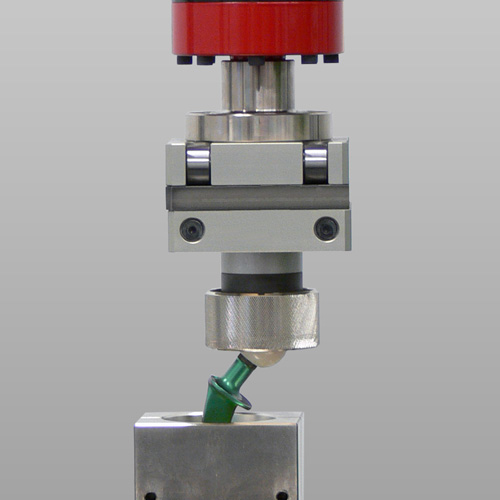
\includegraphics[height=2.5cm]{png/zwick_1}

\textit{Essai de fatigue sur une prothèse de hanche \cite{zwick}}
\end{center}
\end{minipage} \hfill
\begin{minipage}[c]{.2\linewidth}
\begin{center}
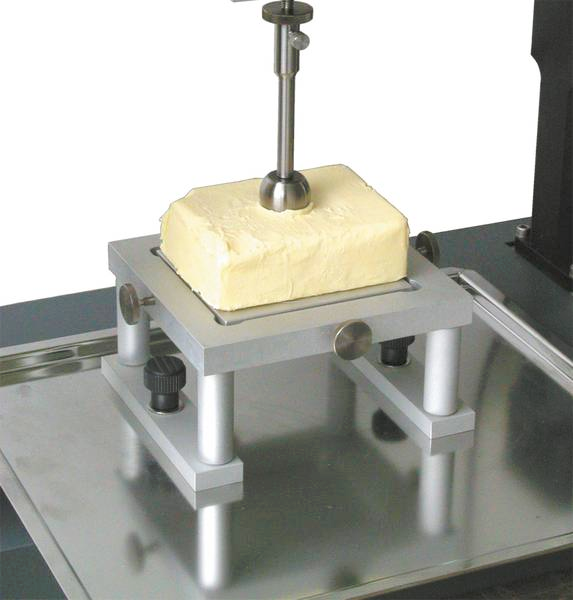
\includegraphics[height=2.5cm]{png/zwick_2}

\textit{Essai de compression d'une motte de beurre \cite{zwick}}
\end{center}
\end{minipage} \hfill
\begin{minipage}[c]{.2\linewidth}
\begin{center}
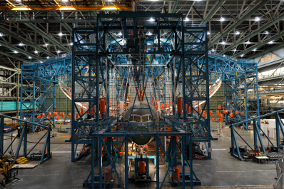
\includegraphics[height=2.5cm]{png/787_p}

\textit{Essai de flexion des ailes sur un Boeing 787}
\end{center}
\end{minipage} \hfill
\begin{minipage}[c]{.2\linewidth}
\begin{center}
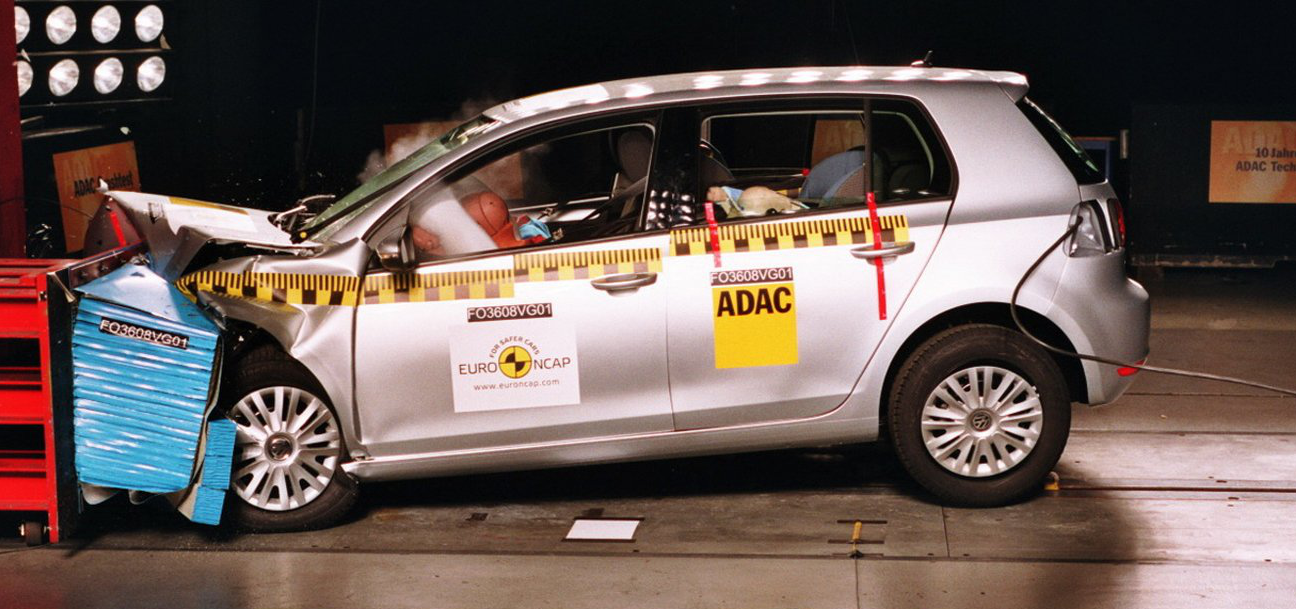
\includegraphics[width=.9\textwidth]{png/crash.png}

\textit{Crash test sur une golf}
\end{center}
\end{minipage}

\vspace{.5cm}

Pour connaître les caractéristiques des matériaux, il est nécessaire de réaliser des essais de caractérisation. La connaissance des propriétés des matériaux permet de faire un choix lors de la conception du produit. D'autres essais peuvent aussi être réalisés sur le produit fini afin de vérifier qu'il satisfait bien le cahier des charges.

\begin{center}
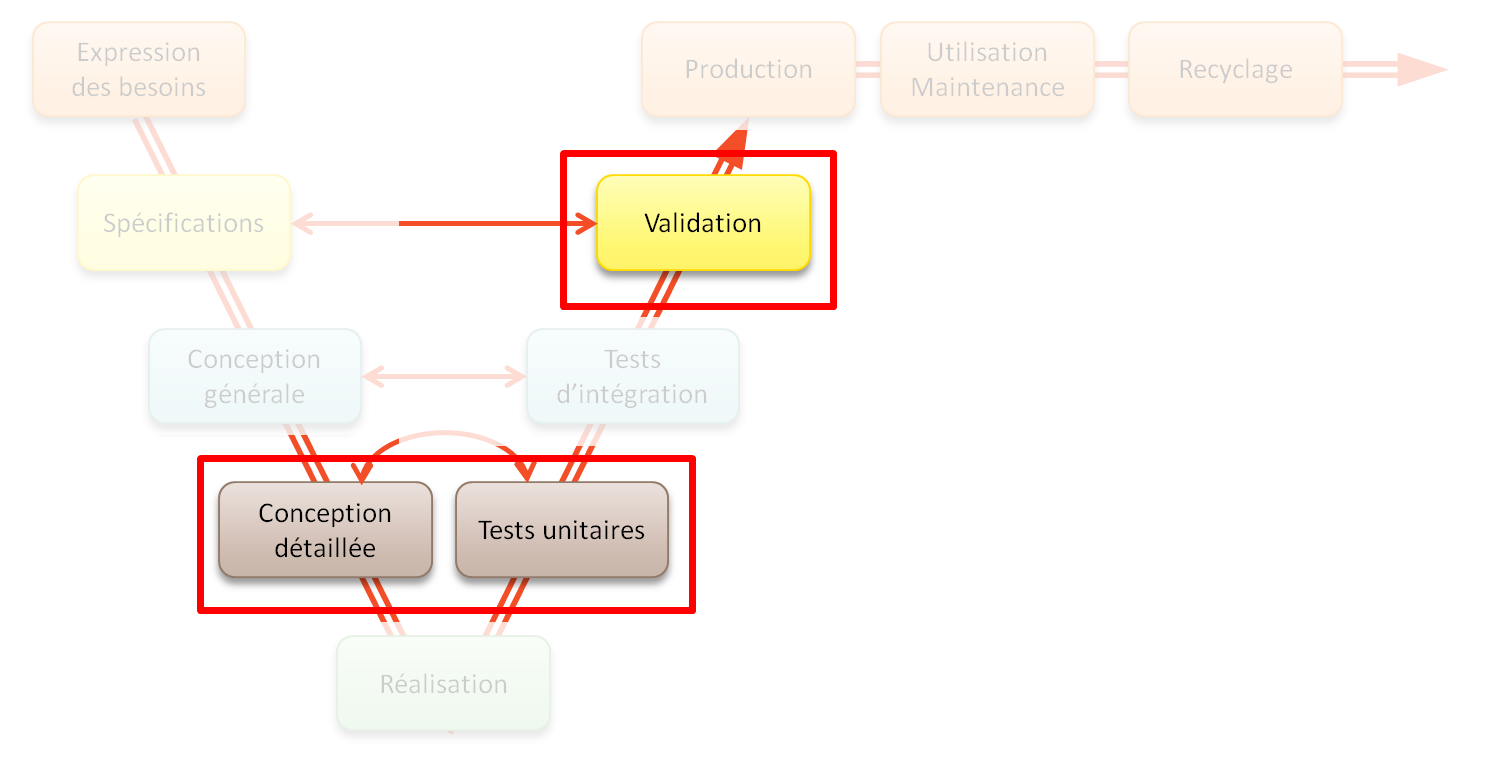
\includegraphics[width=.9\textwidth]{png/cyclev.png}

\textit{Cycle de conception d'un produit}
\end{center}

\begin{prob}
\textsc{Problématique :}

En phase d'avant conception d'un produit, quels sont les critères qui vont permettre de choisir les matériaux à utiliser ?
\end{prob}

\begin{savoir}
\textsc{Savoirs :}
\begin{itemize}
\item Classifier et désigner un matériau métallique.
\item Donner les propriétés d'un matériau métallique.
\item Analyser les essais provenant d'un essai mécanique. 
\end{itemize}
\end{savoir}

%\newpage 

\setlength{\parskip}{0ex plus 0.2ex minus 0ex}
 \renewcommand{\contentsname}{}
 \renewcommand{\baselinestretch}{1}

\tableofcontents

 \renewcommand{\baselinestretch}{1.2}
\setlength{\parskip}{2ex plus 0.5ex minus 0.2ex}

% \vspace{1cm}
\textit{Ce document évolue. Merci de signaler toutes erreurs ou coquilles.}

%\newpage

\section{Caractéristiques mécaniques des matériaux}
%\subsection{Les essais dans le cycle de vie de conception d'un produit}
\subsection{Comportement d'un matériau soumis à de la traction ou de la compression}



\subsubsection{Essai de traction}
\begin{obj}
Le but de l'essai de traction est de déterminer les critères mécanique suivants : 
\begin{itemize}
\item $Re$ (en $MPa$) : limite élastique;
\item $Rm$ (ou $Rr$) (en $MPa$) : limite à la rupture;
\item $E$ (en $MPa$) : module de Young ou module d'élasticité longitudinal;
\item $A\%$ (sans unité) : allongement \%.
\end{itemize}

On parlera ici d'élasticité et de plasiticité des matériaux. 

Il est possible d'évaluer d'autres critères dont nous ne parlerons pas. 
\end{obj}

Les dimensions des éprouvettes utilisées en traction sont normalisées. 

\begin{minipage}[c]{.2\linewidth}
\begin{center}
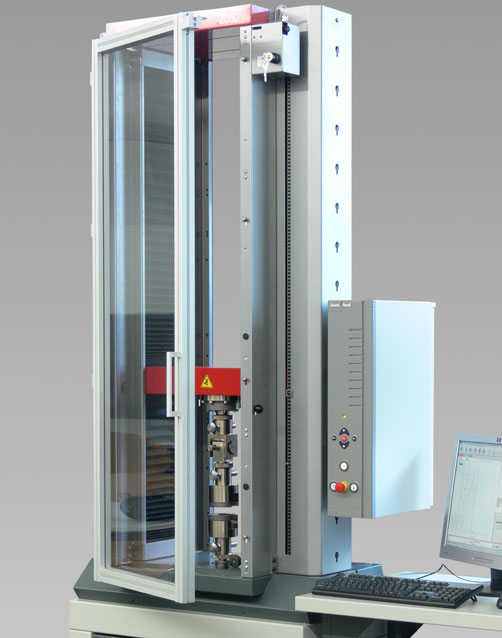
\includegraphics[height=3.5cm]{png/traction}

\textit{Machine de traction}
\end{center}
\end{minipage} \hfill
\begin{minipage}[c]{.2\linewidth}
\begin{center}
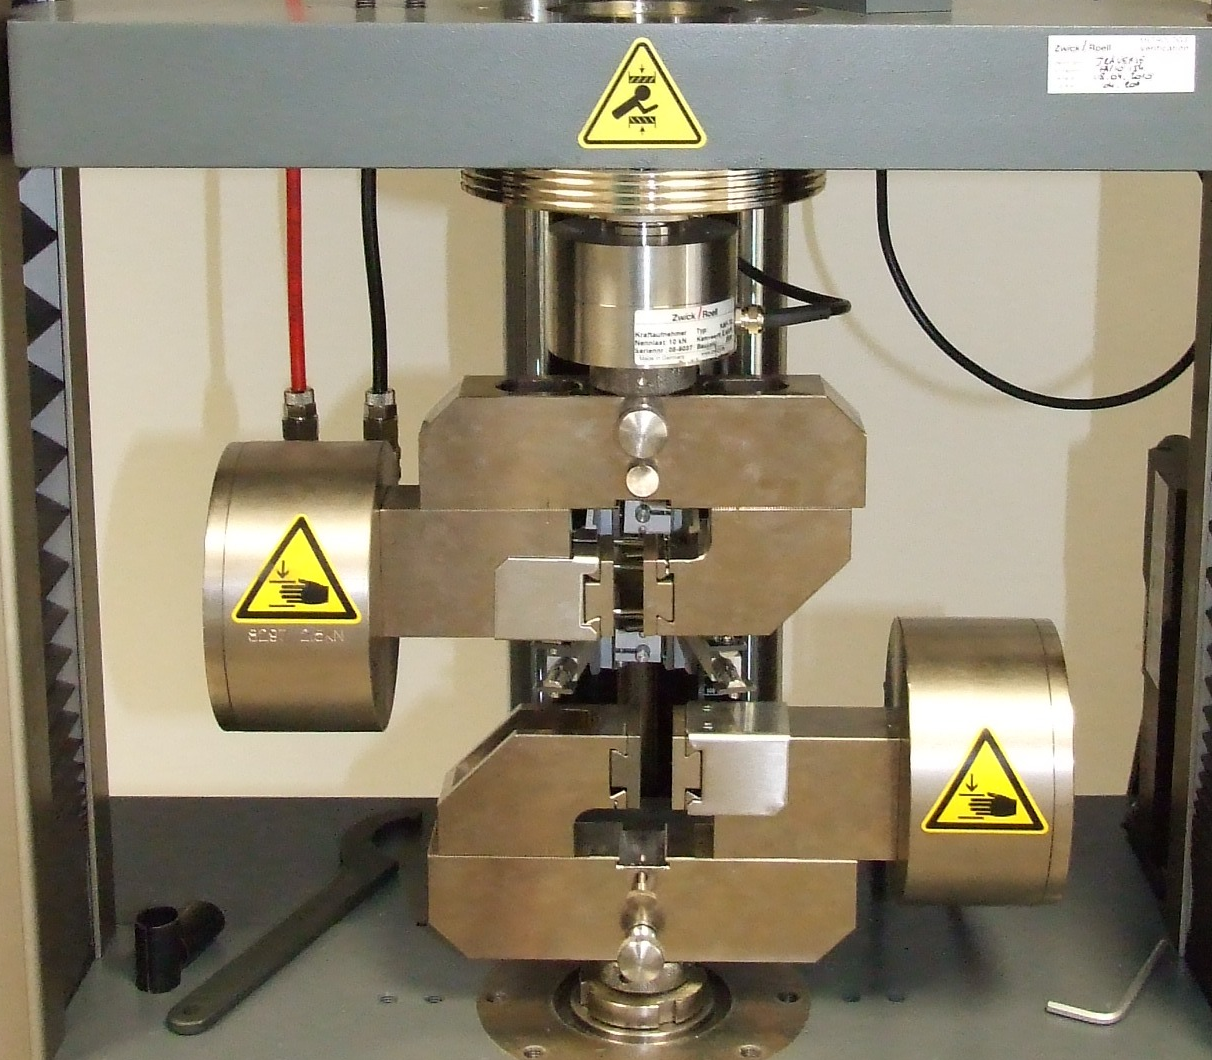
\includegraphics[height=3.5cm]{png/mors}

\textit{Mors de serrage de l'éprouvette}
\end{center}
\end{minipage} \hfill
\begin{minipage}[c]{.2\linewidth}
\begin{center}
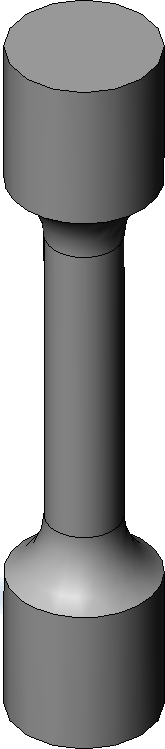
\includegraphics[height=2.5cm]{png/eprouvette_cyl}

\textit{Éprouvette cylindrique}
\end{center}
\end{minipage} \hfill
\begin{minipage}[c]{.2\linewidth}
\begin{center}
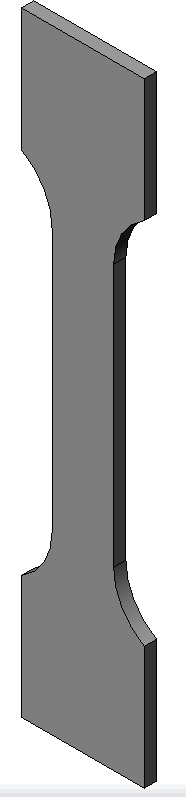
\includegraphics[height=2.5cm]{png/eprouvette_plate}

\textit{Éprouvette plate}
\end{center}
\end{minipage} 

La machine utilisée est une machine de traction. Au cours de l'essai, l'éprouvette est positionnée entre deux mors. Suivant la configuration de la machine, on peut par exemple imposer une vitesse de déplacement entre les mors. On va alors tirer sur l'éprouvette pour parvenir à la rupture, ou non.

La machine mesure d'une part l'effort qu'elle exerce sur l'éprouvette (en $N$). D'autre part le déplacement entre les mors (en $mm$). Les grandeurs mesurées ainsi ont le problème d'être liées à la géométrie de l'éprouvette. Or, les caractéristiques du matériau ne doivent pas dépendre des dimensions d'une pièce. 

En conséquence, le tracé d'un essai de traction aura en abscisse la déformation $\varepsilon$ et en ordonnée la contrainte $\sigma$.


\begin{center}
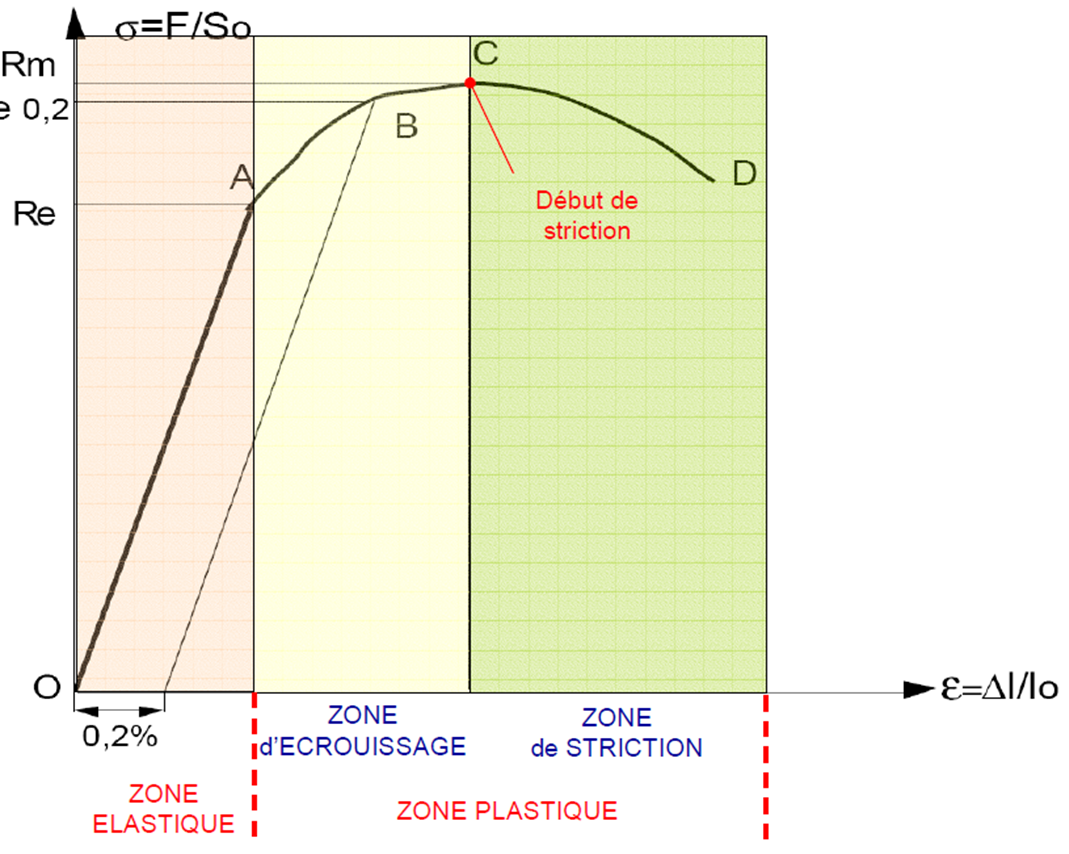
\includegraphics[width=.7\textwidth]{png/courbe_traction}
\end{center}
\begin{defi}
\textbf{La contrainte de traction $\sigma$ est donnée par la formule suivante :}
$$
\sigma  = \dfrac{F}{S_0}
$$
où $\sigma$ est la contrainte de traction en $MPa$, $F$ est l'effort de traction en $N$ et $S_0$ est l'aire de la section de la partie utile de l'éprouvette en $mm^2$.

\textbf{La déformation $\varepsilon$ est donnée par :}
$$
\varepsilon = \dfrac{\Delta L}{L_0}
$$
où $\varepsilon$ est une grandeur sans unité, $\Delta L$ , en $mm$, désigne l'accroissement de distance entre les mors lors de l'essai, $L_0$ désigne la longueur initiale de l'éprouvette.
\end{defi}

\begin{resultat}
\textbf{Loi de Hooke}

Dans la zone élastique, le matériau a un comportement élastique. On définit donc le module de Young $E$ (en $MPa$) (ou module d'élasticité longitudinal) par la relation suivante :
$$
\sigma = E \varepsilon
$$
\end{resultat}


\begin{resultat}
Les caractéristiques de l'essai de traction sont :
\begin{itemize}
\item la contrainte de limite élastique : $R_e = \dfrac{F_e}{S_0}$, $Re$ étant donné en $MPa$;
\item le module d'élasticité longitudinal (ou module de Young), $E$ en $MPa$; 
\item la contrainte de limite à la rupture : $R_m = \dfrac{F_m}{S_0}$, $R_m$ éant donné en $MPa$;
\item l'allongement \% : $A\% = \dfrac{L_u-L_0}{L_0} \cdot 100$.
\end{itemize}
\end{resultat}

\begin{rem}
\textit{Coefficient de Poisson}

Lorsqu'on tire sur une éprouvette, la longueur va s'allonger et la section va se réduire. Dans le cas d'une éprouvette cylindrique, par exemple, on peut donc déterminer :
\begin{itemize}
\item le module d'élasticité longitudinal : $\varepsilon_x = \dfrac{L_u-L_0}{L_0}$;
\item le module d'élasticité transversal : $\varepsilon_y = \dfrac{D_0-D_u}{D_0}$.
\end{itemize}

On appelle $\nu$ coefficient de Poisson. Ce coefficient est constant :
$$
\nu = \dfrac{\varepsilon_y}{\varepsilon_x}
$$

\end{rem}


\begin{rem}
 \textbf{Notion d'écrouissage}

Dans un essai de traction, lorsqu'on applique un effort compris entre la limite élastique et la limite maximale (jusqu'à un effort $F_t$) puis qu'on relâche l'effort, l'éprouvette conserve un allongement permanent. Si on recommence l'essai, on s'aperçoit que la limite élastique du matériau a changé : elle est alors de $\dfrac{F_t}{S}$. Ce procédé est appelé écrouissage. Il permet d'améliorer les performances d'un matériau par déformation plastique. 

\end{rem}

\begin{rem}
 \textbf{Ductilité}

On appelle ductilité la capacité d'un matériau à se déformer plastiquement sans se rompre.

\end{rem}

\begin{exemple}
\textbf{Caractéristiques de quelques matériaux}

\begin{center}
\begin{tabular}{|c|c|c|c|}
\cline{2-4}
\multicolumn{1}{c|}{}& Module de Young $E$ (en $MPa$) & Allongement ($A\%$) & Poisson \\
\cline{2-4}
\hline
Acier & 190 000 à 200 000 & 3\% à 50\% & 0,33 \\ \hline
Aluminium & 70 000 à 80 000 & 5\% à 30\% & 0,33 \\ \hline
Fonte  & 60 000 à 160 000 & 0\% à 20\% & 0,33 \\ \hline
Verre  & 70 000 à 80 000 & 0\% & \\ \hline
\end{tabular}
\end{center}

\end{exemple}

\subsection{Comportement d'un matériau soumis à des efforts ponctuels}
\subsubsection*{Essai de dureté}
\begin{obj}
Le but de l'essai de dureté est de mesurer la capacité d'un matériau à résister à la pénétration par un corps plus dur :
\begin{itemize}
\item $HV$ : dureté Vickers -- pénétration par une pointe pyramidale;
\item $HB$ : dureté Brinell -- pénétration par une bille;
\item $HRb$, $HRc$... : dureté Rockwell -- pénétration par une bille, un cône ...
\item $HSh$ : dureté Shore.
\end{itemize}

On parlera ici de dureté des matériaux. 

\end{obj}

Un protocole de mesure différent existe pour chacun de ces critères.

\paragraph*{Essai de Vickers}
Dans le cas de l'essai de Vickers, une pointe pyramidale en diamant est enfoncé avec un effort $F$ (en $N$) pendant une durée donnée. La pyramide laisse une empreinte de forme carrée dont on mesure les diagonales $d_1$ et $d_2$ grâce à un appareil optique. La moyenne $d$ de $d_1$ et $d_2$ est utilisée pour les calculs de dureté. 

\begin{minipage}[c]{.45\linewidth}
\begin{center}
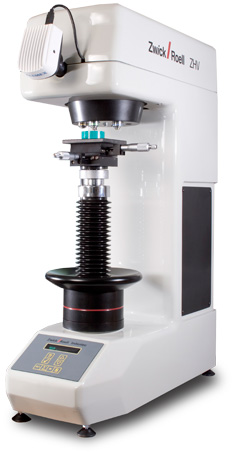
\includegraphics[height=5cm]{png/vickers}

\textit{Machine de dureté ZHV30 Vickers \cite{zwick}}
\end{center}
\end{minipage} \hfill
\begin{minipage}[c]{.45\linewidth}
\begin{center}
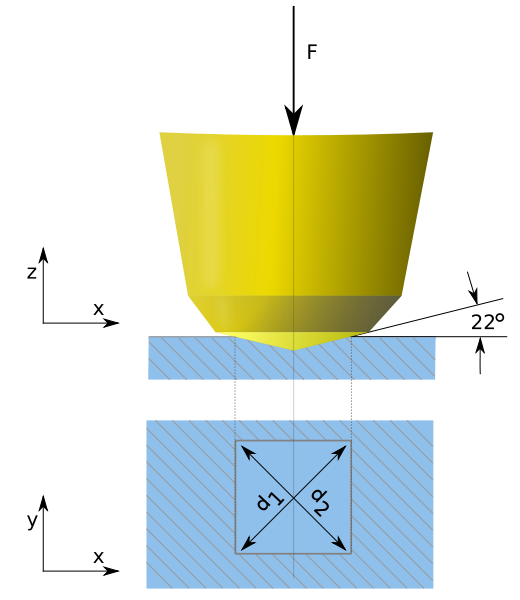
\includegraphics[height=5cm]{png/vickers_2}
\end{center}
\end{minipage}

\begin{resultat}
$$
HV = \dfrac{2F\cdot \sin\left(\dfrac{136^{\text{o}}}{2} \right)}{g\cdot d^2}
\simeq 0,189 \cdot \dfrac{F}{d^2}
$$
\end{resultat}


\paragraph*{Essai de Brinell}

\begin{minipage}[c]{.45\linewidth}
Essai durant lequel une bille de diamètre $D$ est appliquée avec un effort $F$ sur un matériau pendant une durée donnée. On note $d$ le diamètre de l'empreinte sphérique laissée par la bille. 
\end{minipage} \hfill
\begin{minipage}[c]{.45\linewidth}
\begin{center}
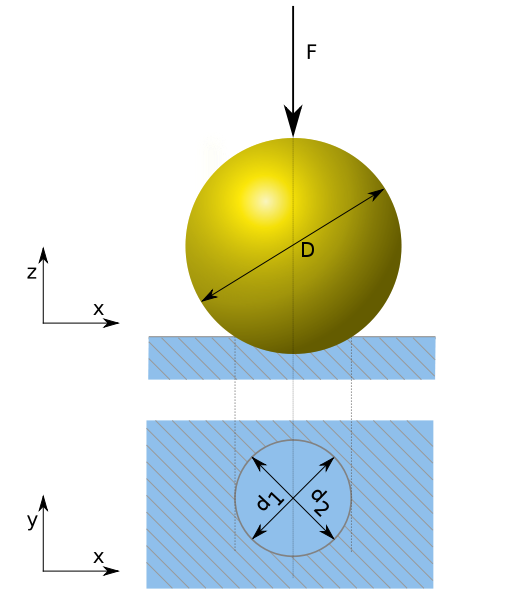
\includegraphics[height=5cm]{png/brinell}
\end{center}
\end{minipage}

\vspace{.5cm}

\begin{resultat}
$$
HB =
 \dfrac{2F}{g\pi D\left( D-\sqrt{D^2-d^2}\right)}
\simeq
0,0649\cdot \dfrac{F}{ D\left( D-\sqrt{D^2-d^2}\right)}
$$
\end{resultat}

\paragraph*{Essai de Rockwell}

Essai basé sur le principe de rémanence. On commence par appliquer un effort de 98 N avec un cône ou une bille en acier trempé. La bille s'enfonce d'une profondeur $p$. On applique un effort supplémentaire et la bille s'enfonce. On relâche alors le second effort et on parvient à une profondeur $P$. Notons $r$ la différence entre $P$ et $p$. 

\begin{center}
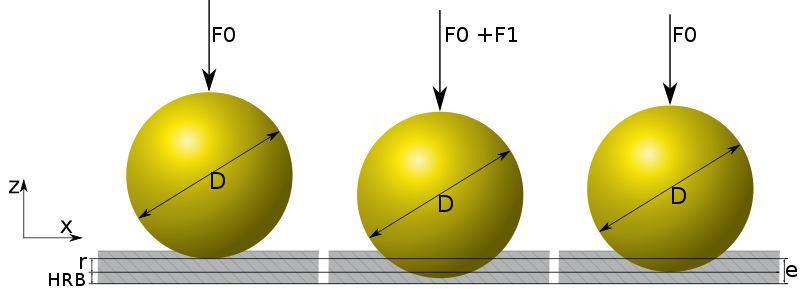
\includegraphics[height=4cm]{png/rockwell}
\end{center}

\begin{resultat}
La valeur de la dureté Rockwell -- bille est donnée par :
$$
HRB = 130 -r
$$
La valeur de la dureté Rockwell -- cône est donnée par :
$$
HRC = 100 -r
$$
\end{resultat}



\paragraph*{Essai de Shore \cite{jb}}

Certains matériaux sont trop élastiques pour conserver une empreinte (caoutchoucs, élastomères). On réalise donc des essais par comparaison. 

Une bille d'acier lâchée d'une hauteur $H$ sur une pièce en acier rebondit d'une hauteur $h$. Cette hauteur sert de référence de mesure. (dureté $HSh = 100$). Cette même bille lâchée d'une même hauteur $H$ sur une autre pièce à tester rebondit d'une hauteur $h'$. On en déduit $HSh$ par rapport à la référence. 


\subsubsection*{Table de conversion}
\begin{center}
\begin{tabular}{|c|c|c|c|c|}
\hline 
$R_m$ ($MPa$) & $HB$ & $HV$ & $HRB$ & $HRC$\\
\hline \hline
285 & 86 & 90 & & \\
\hline
385 & 114 & 120 & 66,7 & \\ \hline
510 & 152 & 160 & 81,7 & \\ \hline
800 & 238 & 250 & 99.5 &\\ \hline
820 & 242 & 255 &  & 23.1 \\ \hline
995 & 295 & 310 &  & 31.0 \\ \hline
1290 & 380 & 400 &  & 40.8 \\ \hline
1995 & 570 & 600 &  & 55.2 \\ \hline
2180 & 618 & 650 &  & 57.8 \\ \hline
\end{tabular}
\end{center}

\subsection{Comportement d'un outil soumis à un choc}

\subsubsection{Essai de Charpy}

\begin{obj}
On appelle résilience $K$ d'un matériau sa capacité à résister aux chocs. On appelle \textbf{résilience} la capacité d'un matériau à résister aux chocs. 
\end{obj}

Les éprouvettes utilisées sont entaillées et normalisées. 

L'essai peut être réalisé sur un mouton de Charpy. Au cours de cet essai une éprouvette est positionnée sur 2 appuis fixes. La machine est constituée d'un pendule au bout duquel est positionné un couteau. Le couteau est lancé d'une hauteur donnée et vient impacter l'éprouvette. On mesure alors la hauteur atteinte par le pendule après impact. Le paramètre $K$ est donné par la différence entre l'énergie potentielle initiale du mouton et l'énergie potentielle après impact. 


\begin{minipage}[c]{.2\linewidth}
\begin{center}
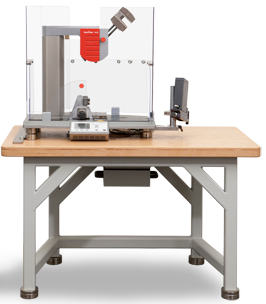
\includegraphics[height=3.5cm]{png/mouton_1}

\textit{Mouton de Charpy -- 50 Joules}
\end{center}
\end{minipage} \hfill
\begin{minipage}[c]{.2\linewidth}
\begin{center}
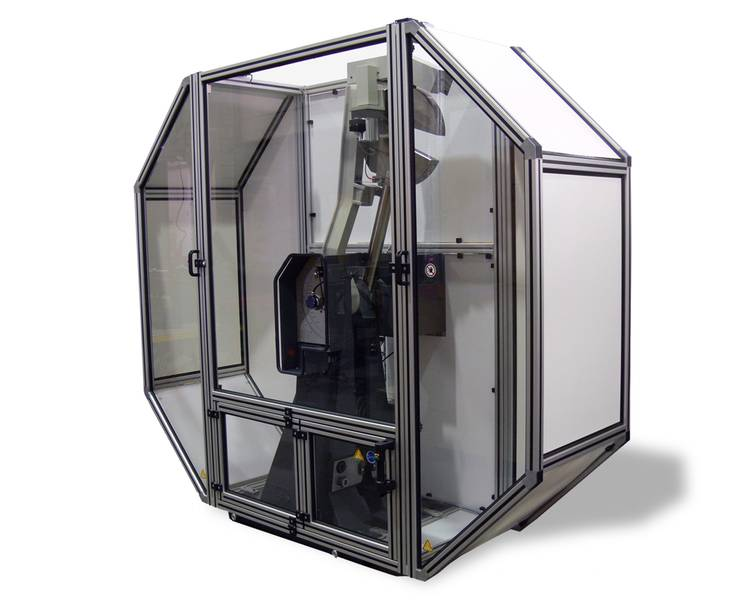
\includegraphics[height=3.5cm]{png/mouton_2}

\textit{Mouton de Charpy -- 750 Joules}
\end{center}
\end{minipage} \hfill
\begin{minipage}[c]{.2\linewidth}
\begin{center}
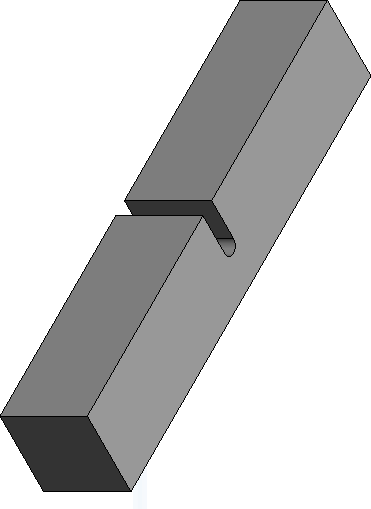
\includegraphics[height=2.5cm]{png/eprouvette_U}

\textit{Éprouvette avec entaille en U}
\end{center}
\end{minipage} \hfill
\begin{minipage}[c]{.2\linewidth}
\begin{center}
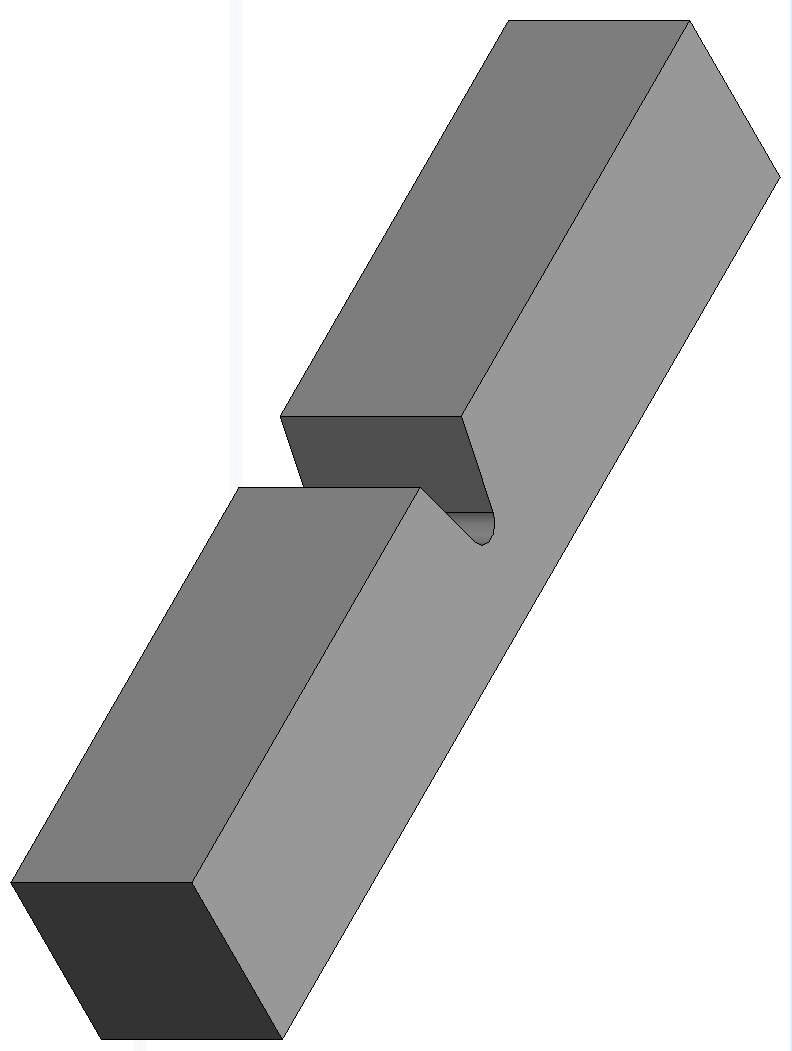
\includegraphics[height=2.5cm]{png/eprouvette_V}

\textit{Éprouvette avec entaille en V}
\end{center}
\end{minipage} 

\begin{minipage}[c]{.45\linewidth}
Si on considère un pendule de masse $M$ lancé à une hauteur $h$. L'énergie potentielle de pesanteur d'origine est donnée par : $W_0 = Mgh$. Après lancement du mouton et rupture de l'éprouvette, le pendule monte a une hauteur $h'$. L'énergie potentielle de pesanteur est alors donnée par $W_1=Mgh'$.
\end{minipage} \hfill
\begin{minipage}[c]{.45\linewidth}
\begin{center}
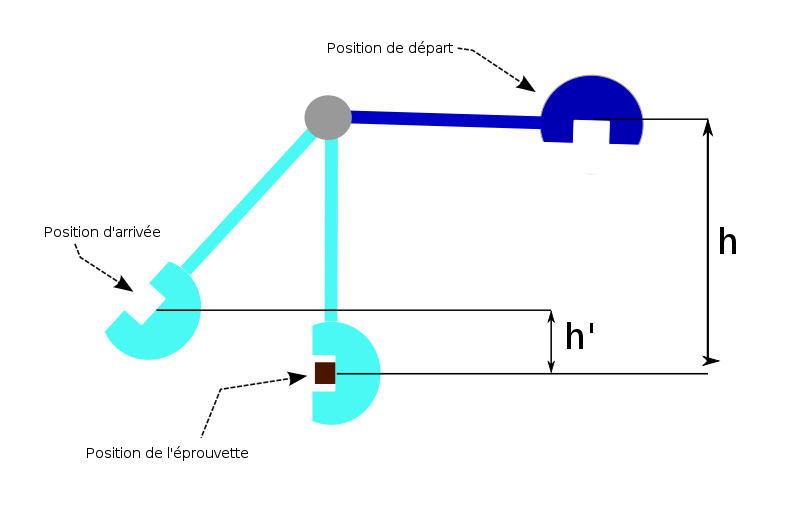
\includegraphics[width=.9\textwidth]{png/charpy_2}

\end{center}
\end{minipage}

\begin{resultat}
\textbf{Coefficient de résilience $KCU$ ou $KCV$ :}

$$KCU = \dfrac{W}{S_0} = \dfrac{Mg\left(h-h' \right)}{S_0}$$
\begin{itemize}
\item $KCU$ en $J/cm^2$;
\item $M$ en $kg$;
\item $g=9,81\;m/s^2$;
\item $W$ en Joules;
\item $S_0$ en $cm^2$;
\item $H$ en $m$.
\end{itemize}


\end{resultat}
 
\subsection{Comportement d'un outil soumis à des efforts cycliques}
\subsubsection{Essai de fatigue \cite{jb}}

Lorsqu'une pièce subit des sollicitations alternées et si le nombre des alternances est important, la rupture de la pièce intervient généralement sans que la contrainte ait atteint la limite élastique du matériau. Pour prévoir le comportement des structures et tenir compte de ce phénomène, on réalise des essais appelés "essais de fatigue". 

Il existe de nombreux essais de fatigue qui permettent d'évaluer la capacité des pièces de formes diverses à résister à différentes sollicitations. Cette capacité de résister s'appelle endurance.

\begin{obj}
\textbf{Principe de l'essai}

L'essai de fatigue consiste à imposer à une pièce une force ou un déplacement variable dans le temps. Les essais les plus courants consistent à imposer des cycles d'efforts périodiques sinusoïdaux. On mesure le nombre d'alternances supportées. 

\end{obj}


\begin{exemple}
\textbf{Essais de flexion}

\end{exemple}

Il existe de nombreuses autres sortes de sollicitations pour les essais de fatigue :
\begin{itemize}
\item essai de traction compression;
\item essai de torsion ...
\end{itemize}


\paragraph*{Conduite d'un essai de fatigue}

Considérons un lot d'éprouvettes identiques et appliquons à chacune d'elles des efforts périodiques, de fréquence constante, mais avec une amplitude d'effort différente pour chaque éprouvette. 

La première éprouvette sera soumise à un effort maximal correspondant à une contrainte $\sigma_{maxi} = R_m$. Elle se rompt normalement pour un cycle $Ncy = 1$. 

La deuxième éprouvette sera soumise à un effort maximal correspondant à une contrainte $\sigma < R_m$. On note $Ncy$ le nombre de cycles ayant entraîné la rupture. 

Pour les éprouvettes suivantes, l'amplitude de l'effort sera de plus en plus faible et on notera pour chaque essai le nombre de cycles ayant entraîné la rupture de chacune des éprouvettes. 

Ces résultats sont représentés sur un diagramme avec $Ncy$ en abscisse (échelle logarithmique) et $\sigma$ en ordonnée. A chaque éprouvette correspond un point du diagramme. 

La courbe moyenne qui relie les différents points Mi s'appelle \textbf{courbe de Wöhler}.


\begin{minipage}[c]{.45\linewidth}
\begin{center}
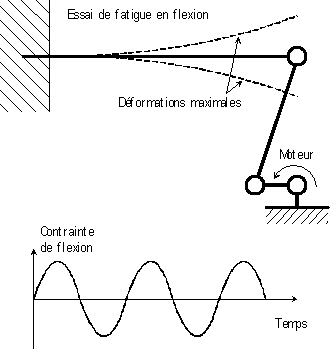
\includegraphics[width=.9\textwidth]{png/wohler_2}
\end{center}
\end{minipage}\hfill
\begin{minipage}[c]{.45\linewidth}
\begin{center}
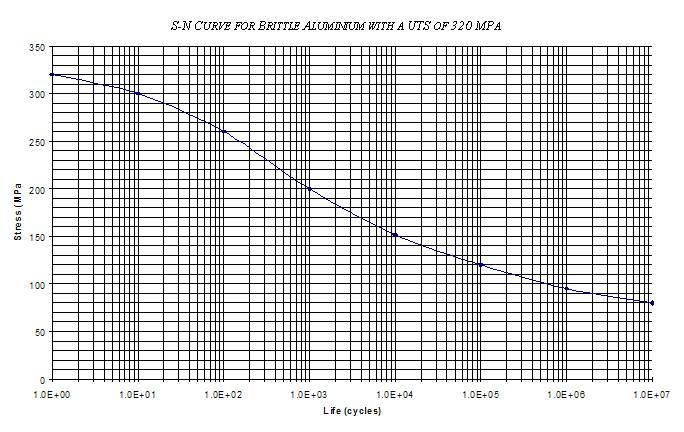
\includegraphics[width=.95\textwidth]{png/wohler}
\end{center}
\end{minipage}

\vspace{.5cm}

La limite asymptotique est appelée \textbf{limite de fatigue}. Cette asymptote ne peut pas être déterminée avec précision expérimentalement. On définit donc une limite pratique conventionnelle $fp$.

Pour les alliages ferreux, le nombre de cycle est de l'ordre de $3\cdot 10^7$ cycles. Il est de l'ordre $10^8$ pour les alliages d'aluminium.


\paragraph*{Paramètres influant sur la résistance à la fatigue d'une pièce mécanique}

La forme des pièces (épaulement, rainures, gorges, trous, angles vifs ...) constituent des zones de concentration de contraintes qui diminuent la résistance à la fatigue. 

\begin{exemple}
Une gorge de diamètre 6 mm sur une arbre de diamètre 30 mm amène à diviser par 2 la contrainte maximale admissible.
\end{exemple}

L'état de surface, et donc les rayures, constituent des amorces de rupture des pièces mécaniques.
Les dimensions aussi.

La fréquence de sollicitation n'a que peu d'influence sur la durée de vie. 

\section{Désignation des matériaux}
\subsection{Désignation des aciers}
On distingue plusieurs familles d'acier : 
\begin{itemize}
\item les aciers non alliés d'usage général ou spéciaux;
\item les aciers faiblement alliés pour lesquels aucun élément d'addition ne dépasse 5\%;
\item les aciers fortement alliés.
\end{itemize}
\subsubsection{Aciers non alliés}
\begin{resultat}
\begin{center}
\texttt{Lettre \hspace{1cm} Limite élastique $Re$ en $MPa$}
\end{center}

Concernant la lettre :
\begin{itemize}
\item $S$ : acier d'usage général;
\item $E$ : acier pour construction mécanique. 
\end{itemize}
\end{resultat}

\begin{exemple}

\begin{minipage}[c]{.3\linewidth}
\begin{center}
$ S\; 235 $
\end{center}
\end{minipage} \hfill
\begin{minipage}[c]{.6\linewidth}
S : acier d'usage général. Limite élastique : $235\;MPa$
\end{minipage}

\begin{minipage}[c]{.3\linewidth}
\begin{center}
$ E\; 335 $
\end{center}
\end{minipage} \hfill
\begin{minipage}[c]{.6\linewidth}
E : acier pour la construction mécanique. Limite élastique : $335\;MPa$
\end{minipage}
\end{exemple}

\begin{rem}
On peut rencontrer le préfixe $G$ devant la désignation. Cela signifie que l'acier est moulé : 
\begin{minipage}[c]{.3\linewidth}
\begin{center}
$ GE\; 295 $
\end{center}
\end{minipage} \hfill
\begin{minipage}[c]{.6\linewidth}
GE : Acier moulé pour la construction mécanique. Limite élastique : $295\;MPa$
\end{minipage}
\end{rem}



\subsubsection{Aciers non alliés}
\begin{resultat}
Ces aciers ont un pourcentage de manganèse inférieur à 1\%. Ils sont notés ainsi :

\begin{center}
\texttt{C \hspace{1cm} 100x le \% de carbone}
\end{center}

\end{resultat}

\begin{exemple}
\begin{minipage}[c]{.3\linewidth}
\begin{center}
$ C\; 60$
\end{center}
\end{minipage} \hfill
\begin{minipage}[c]{.6\linewidth}
\begin{itemize}
\item C : Acier non allié. 
\item 60 : 0,6\% de carbone. 
\end{itemize}
\end{minipage}
\end{exemple}

\subsubsection{Aciers faiblement alliés}
\begin{resultat}
Ces aciers ont un pourcentage de manganèse inférieur à 1\%. Le pourcentage des autres éléments d'addition ne dépasse pas 5\%. Ils sont notés ainsi :


\begin{minipage}[c]{.3\linewidth}
\begin{center}
\texttt{100x le \% de carbone}
\end{center}
\end{minipage} \hfill
\begin{minipage}[c]{.3\linewidth}
\begin{center}
\texttt{Liste des éléments d'addition}
\end{center}
\end{minipage} \hfill
\begin{minipage}[c]{.3\linewidth}
\begin{center}
\texttt{Liste respective des pourcentages (à un coef. diviseur près)}
\end{center}
\end{minipage} 

\end{resultat}

\begin{center}
\begin{tabular}{|c|c|c||c|c|c||c|c|c|}
\hline
Élément	 & Symb. & Multipli. & Élément & Symb. & Multipli. & Élément & Symb. & Multipl. \\
\hline
\hline
Aluminium & $Al$ & 10 & Magnésium & $Mg$ && Soufre & $S$ & 100 \\ \hline
Beryllium  & $Be$ & 10 & Manganèse & $Mn$ & 4 & Strontium & $Sr$	& \\ \hline
Bore	       & $B$ & 1000 & Molybdène & $Mo$ & 10 & Tantale & $Ta$ & 10 \\ \hline
Cérium    & $Ce$ & 100 & Nickel & $Ni$ & 4 & Titane & Ti & 10 \\ \hline
Chrome   & $Cr$ & 4 & Niobium & Nb & 10 & Tungstène & $W$ & 4 \\ \hline
Cobalt     & $Co$  & 4 & Plomb & Pb & 10 & Vanadium	 & $V$ & 10 \\ \hline
Cuivre     & $Cu$ & 10 & Phosphore & P & 100 & Zinc & $Zn$ &\\ \hline
Étain	       &$Sn$ && Silicium & $Si$ & 4 & Zirconium & $Zr$ & 10 \\
\hline
\end{tabular}
\end{center}


\begin{exemple}
\begin{minipage}[c]{.3\linewidth}
\begin{center}
$ 42\; Cr\; Mo\; 6$
\end{center}
\end{minipage} \hfill
\begin{minipage}[c]{.6\linewidth}
\begin{itemize}
\item Acier faiblement allié
\item 0,42 \% de carbone
\item 1,5\% de chrome 
\item des traces de molybdène
\end{itemize}
\end{minipage}
\end{exemple}


\subsubsection{Aciers fortement alliés}
\begin{resultat}
Le pourcentage d'un des éléments d'addition dépasse  5\%. Ils sont notés ainsi :


\begin{minipage}[c]{.1\linewidth}
\begin{center}
\texttt{X}
\end{center}
\end{minipage} \hfill
\begin{minipage}[c]{.2\linewidth}
\begin{center}
\texttt{100x le \% de carbone}
\end{center}
\end{minipage} \hfill
\begin{minipage}[c]{.2\linewidth}
\begin{center}
\texttt{Liste des éléments d'addition}
\end{center}
\end{minipage} \hfill
\begin{minipage}[c]{.3\linewidth}
\begin{center}
\texttt{Liste respective des pourcentages des éléments d'addition séparés par des tirets}
\end{center}
\end{minipage} 
\end{resultat}


\begin{exemple}
\begin{minipage}[c]{.3\linewidth}
\begin{center}
$ X\; 5\;  Cr\; Ni\; 18-10$
\end{center}
\end{minipage} \hfill
\begin{minipage}[c]{.6\linewidth}
\begin{itemize}
\item Acier fortement allié
\item 0,05\% de carbone
\item 18\% de chrome 
\item 10\% de nickel
\end{itemize}
\end{minipage}
\end{exemple}

\subsection{Désignation des fontes}

\subsubsection{Fontes à graphites lamellaire}

\begin{resultat}
Le graphite apparaît sous forme de lamelles. Elles sont facilement obtenus. Elles offrent peu de résistance aux chocs et à l'extension.


\begin{minipage}[c]{.3\linewidth}
\begin{center}
\texttt{EN-GJL}
\end{center}
\end{minipage} \hfill
\begin{minipage}[c]{.5\linewidth}
\begin{center}
\texttt{Résistance à la rupture $Rm$ en $MPa$}
\end{center}
\end{minipage} 
\end{resultat}


\begin{exemple}
\begin{minipage}[c]{.3\linewidth}
\begin{center}
$ EN-GJL-250$
\end{center}
\end{minipage} \hfill
\begin{minipage}[c]{.6\linewidth}
\begin{itemize}
\item Fonte à graphite lamellaire
\item $Rm = 250\; MPa$
\end{itemize}
\end{minipage}
\end{exemple}

\subsubsection{Fontes malléables}

\begin{resultat}
Fontes malléables à c\oe{}ur blanc :

\begin{minipage}[c]{.3\linewidth}
\begin{center}
\texttt{EN-GJMW}
\end{center}
\end{minipage} \hfill
\begin{minipage}[c]{.3\linewidth}
\begin{center}
\texttt{Résistance à la rupture $Rm$ en $MPa$}
\end{center}
\end{minipage} \hfill
\begin{minipage}[c]{.3\linewidth}
\begin{center}
\texttt{Allongement \%}
\end{center}
\end{minipage} 

Fontes malléables à c\oe{}ur noir :

\begin{minipage}[c]{.3\linewidth}
\begin{center}
\texttt{EN-GJMB}
\end{center}
\end{minipage} \hfill
\begin{minipage}[c]{.3\linewidth}
\begin{center}
\texttt{Résistance à la rupture $Rm$ en $MPa$}
\end{center}
\end{minipage} \hfill
\begin{minipage}[c]{.3\linewidth}
\begin{center}
\texttt{Allongement \%}
\end{center}
\end{minipage} 


\end{resultat}


\begin{exemple}
\begin{minipage}[c]{.3\linewidth}
\begin{center}
$ EN-GJMW\;400-5$
\end{center}
\end{minipage} \hfill
\begin{minipage}[c]{.6\linewidth}
\begin{itemize}
\item Fonte malléable à c\oe{}ur blanc
\item $Rm = 400\; MPa$
\item $A\%\; 5$
\end{itemize}
\end{minipage}

\begin{minipage}[c]{.3\linewidth}
\begin{center}
$ EN-GJMB\;600-3$
\end{center}
\end{minipage} \hfill
\begin{minipage}[c]{.6\linewidth}
\begin{itemize}
\item Fonte malléable à c\oe{}ur noir
\item $Rm = 600\; MPa$
\item $A\%\; 3$
\end{itemize}
\end{minipage}
\end{exemple}


\subsubsection{Fontes à graphite sphéroïdal}

\begin{resultat}

\begin{minipage}[c]{.3\linewidth}
\begin{center}
\texttt{EN-GJS}
\end{center}
\end{minipage} \hfill
\begin{minipage}[c]{.3\linewidth}
\begin{center}
\texttt{Résistance à la rupture $Rm$ en $MPa$}
\end{center}
\end{minipage} \hfill
\begin{minipage}[c]{.3\linewidth}
\begin{center}
\texttt{Allongement \%}
\end{center}
\end{minipage} 


\end{resultat}


\begin{exemple}
\begin{minipage}[c]{.3\linewidth}
\begin{center}
$ EN-GJS\;600-3$
\end{center}
\end{minipage} \hfill
\begin{minipage}[c]{.6\linewidth}
\begin{itemize}
\item Fonte à graphite sphéroïdal
\item $Rm = 600\; MPa$
\item $A\%\; 3$
\end{itemize}
\end{minipage}

\end{exemple}




\subsection{Désignation des alliages d'aluminium}

\subsubsection{Aluminium pur}

\begin{resultat}

\begin{minipage}[c]{.3\linewidth}
\begin{center}
\texttt{Al}
\end{center}
\end{minipage} \hfill
\begin{minipage}[c]{.3\linewidth}
\begin{center}
\texttt{\% d'aluminium}
\end{center}
\end{minipage} 
\end{resultat}


\begin{exemple}
\begin{minipage}[c]{.3\linewidth}
\begin{center}
$ Al \, 99,5$
\end{center}
\end{minipage} \hfill
\begin{minipage}[c]{.6\linewidth}
\begin{itemize}
\item Alliage d'aluminium à 99,5\%.
\end{itemize}
\end{minipage}

\end{exemple}



\subsubsection{Alliages d'aluminium}

\begin{resultat}

\begin{minipage}[c]{.3\linewidth}
\begin{center}
\texttt{Al}
\end{center}
\end{minipage} \hfill
\begin{minipage}[c]{.3\linewidth}
\begin{center}
\texttt{Élément d'addition accompagné de son \%}
\end{center}
\end{minipage} 

\end{resultat}


\begin{exemple}
\begin{minipage}[c]{.3\linewidth}
\begin{center}
$Al\; Si\; 10\; Mg$
\end{center}
\end{minipage} \hfill
\begin{minipage}[c]{.6\linewidth}
\begin{itemize}
\item Alliage d'aluminium
\item 10\% de silicium
\item des traces de magnésium
\end{itemize}
\end{minipage}

\end{exemple}




\subsection{Désignation des alliages de cuivre}
Les désignations utilisées pour l'aluminium restent en vigueur en remplaçant $Al$ par $Cu$.


\subsection{Influence des éléments d'addition}

\begin{center}
\begin{tabular}{|p{.25\textwidth}|c|c|c|c|c|c|c|c|c|c|}
\hline
Caractéristiques & \multicolumn{10}{c|}{Éléments d'addition} \\
\hline
& $Cr$ & $Co$ & $Mn$ & $Mo$ & $Ni$ & $Ti$ & $W$ & $V$ & $P$ & $Si$ \\ \hline
Trempabilité & ++ & - & +++&+++ &++&++&+++&+++&+&++ \\ \hline
Durcissement ferrite&+&+++&++&+&+&&&+&++&+ \\ \hline
%Revenu&&&&&&&&&& \\ \hline
Dureté et résistance mécanique&++&+&++&++&+&+&+&+&+&+ \\ \hline
Ductilité &-&&+&+&+&+&+&+&-&- \\ \hline
Résilience&+&+&+&+&+&+&+&+&& \\ \hline\hline
Soudabilité &-&&+&+&&&&+&&- \\ \hline
Forgeabilité &&&+&+&+&+&&+&& \\ \hline
Usinabilité &-&+&&&-&&&&+& -\\ \hline
Résistance à la corrosion et la chaleur &++&&&+&+&+&+&&&- \\ \hline

\end{tabular}
\end{center}


\begin{thebibliography}{2}
\bibitem{zwick}{\url{http://www.zwick.fr/fr.html}}

%\bibitem{acier}{\url{http://www.lefigaro.fr/medias/2008/12/18/47e0e366-cd2c-11dd-882f-4b99bc2f9b71.jpg}}
%\bibitem{composite}{\url{http://fr.gurit.com/benefits-of-composite-materials.aspx}}
%\bibitem{verre}{\url{http://www.vezenobres.info/partenaires.htm}}
%\bibitem{ldr}{LDR Médical \url{http://fr.ldrmedical.com/Produits/Thoraco-lombaire/MobidiscProthèsededisquelombaire}}
%\bibitem{dent}{Protilab \url{http://www.protilab.com/fr/prothese/7/Couronne+sur+implant}}
%\bibitem{wafer}{\url{http://www.efficacite-electrique.fr/2012/03/usa-semi-conducteurs-plus-compacts-meilleure-efficacite-electrique/}}
%\bibitem{carter}{\url{http://www.directindustry.fr/prod/sermes/moto-reducteurs-electriques-a-vis-sans-fin-a-carter-en-fonte-7542-424078.html}}
%\bibitem{fer}{\url{http://www.zpag.net/Tecnologies_Indistrielles/Metaux_Ferreux.htm}}
%\bibitem{a350}{© Airbus S.A.S.}

\bibitem{rb}{Supports de cours de Renan Bonnard,PTSI, Lycée Newton, Clichy la Garenne}
\bibitem{jb}{Supports de cours de Joël Boiron, PTSI, Lycée Gustave Eiffel, Bordeaux}
\bibitem{wikipedia}{Wikipédia, Dureté (matériau) --- Wikipédia{,} l'encyclopédie libre, 2012, \url{
http://fr.wikipedia.org/w/index.php?title=Duret\%C3\%A9_(mat\%C3\%A9riau)\&oldid=83575804}}
%\bibitem{mc}{Supports de cours de Maryline Carrez, Lycée Jules Haag, Besançon}
%\bibitem{pf}{Supports de cours de Philippe Fichou, Lycée Vauban, Brest \url{http://philippe.fichou.pagesperso-orange.fr/documents/liaisoncomplete2003.pdf}}
%\bibitem{jpp}{Supports de cours de Jean-Pierre Pupier, Lycée Rouvière, Toulon}


\end{thebibliography}

\end{document}